\documentclass[12pt]{exam}
\usepackage[hon]{template-for-exam}
\usepackage{tikz,ifthen}
\usepackage[margin=0.5in]{geometry}
\usepackage{graphicx}
\footer{}{}{}
\header{}{}{}
\shadedsolutions
%\printanswers



\begin{document}

\def\mystrut{\protect\rule[-2.2ex]{0ex}{2.2ex}} 
\qformat{ \textbf{Task \#\thequestion}
  \ifthenelse{\equal{\thequestion}{\thequestiontitle}}
    {}
    {: \emph{\thequestiontitle}}
  \mystrut  \hfill}
\begin{questions}

  \Large

  \question 
    A baseball pitcher throws a baseball with a speed of 43~m/s.  Estimate the acceleration of the ball during the throwing motion.  In throwing the baseball, the pitcher accelerates it through a displacement of about 3.5~m.

    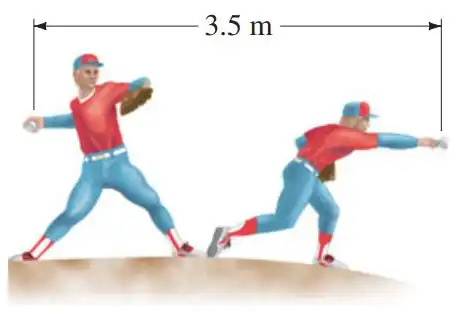
\includegraphics[width=6cm]{baseball.png}

    \begin{solution}
      264~m/s$^2$
    \end{solution}
    
    {\tiny This problem is based on Ch 2, Problem 25 in Giancolli \emph{Physics}, 7th ed.}
    \vs\hrule\vs
  \question
    A world-class sprinter can reach a top speed of 11.5~m/s in the first 18.0~m of a race.  What is the average acceleration of this sprinter?  How long does it take her to reach that speed?

    \begin{solution}
      3.67 m/s$^2$; 3.13~s
    \end{solution}

    {\tiny This problem is based on Ch 2, Problem 26 in Giancolli \emph{Physics}, 7th ed.}
    \vs\hrule\vs
  \question
    A car slows down uniformly from a speed of 28.0~m/s to rest in 8.00~s.  How far did it travel in that time?

    \begin{solution}
      $a=-3.5$~m/s$^2$; 112~m
    \end{solution}
    
    {\tiny This problem is based on Ch 2, Problem 27 in Giancolli \emph{Physics}, 7th ed.}
    \vs\hrule\vs
  \question
    You are driving in a car going 26~m/s.  All of a sudden, you see an obstacle in the road.  Calculate the stopping distance of your car.  Assume that your human reaction time is 0.40~seconds and the deceleration applied by the brakes is 3.0~m/s$^2$.

    \begin{solution}
      $0.4 \cdot 26 = 10.4$; $26^2/(2\cdot 3.0) = 112.7$; total distance = 123.1~m
    \end{solution}
    
    {\tiny This problem is based on Ch 2, Problem 31 in Giancolli \emph{Physics}, 7th ed.}
 \end{questions}




\end{document}